\documentclass{ecai2010}
\usepackage{times}
\usepackage{graphicx}
\usepackage{latexsym, epstopdf, pgfplots, setspace}
\usepackage[algo2e, noend, noline, linesnumbered]{algorithm2e}
\DontPrintSemicolon
\newcommand{\pushline}{\Indp}% Indent
\newcommand{\popline}{\Indm}
\newcommand{\sgn}{\mathop{\mathrm{sgn}}}
\ecaisubmission   % inserts page numbers. Use only for submission of paper.
                  % Do NOT use for camera-ready version of paper.

\begin{document}

\title{Quality-based rewards for Monte-Carlo Tree Search simulations}

\author{Tom Pepels \and Marc Lanctot \and Mark~H.~M. Winands \institute{Maastricht University,
The Netherlands, email: \{tom.pepels,marc.lanctot,m.winands\}@maastrichtuniversity.nl} }

\maketitle
\bibliographystyle{ecai2010}

\begin{abstract}
In this paper methods for assessing the a posteriori quality of Monte-Carlo simulations are introduced. We show that altering the rewards of simulated play-outs in Monte-Carlo Tree Search based on their assessed quality improves results in five different 2-player boardgames. To achieve these results we propose two novel enhancements, the \emph{Qualitative Bonus} and the \emph{Relative Bonus}. The former relies on an uncomplicated heuristic evaluation of the game's terminal state, whereas and the latter relies on the total number of moves made during any simulated play-out. The proposed enhancements lead to a considerable performance increase in all five domains discussed.
\end{abstract}

%-------------------------------------------------------------------
\section{Introduction}
\label{sec:intro}
Monte-Carlo Tree Search (MCTS) depends on the results of numerous simulations, each simulation consists of two parts, 1) the selection step, where moves are selected and played according to the UCT selection policy, and 2) the play-out step, where moves are played according to a (random) simulation strategy. At the end of each play-out a terminal state is reached and the result $r_t$, for simulation $t$ is usually expressed numerically in some discrete range, e.g. $r_t \in [-1, 0, 1]$ a loss, draw or win, respectively, and backpropagated along the tree from the expanded leaf to the root node. MCTS then collects these rewards at the nodes on the first ply, and a final move to play is selected based on either the number of visits, the average reward, or a combination of the two \cite{chaslot2008progressive}.

Other techniques for rewarding simulations have been proposed \cite{Winands2010a}, where play-outs are cut-off early and their state heuristically evaluated. Furthermore, evaluating the final score of a game has shown to improve results in games that base the winning player on the one with the highest score \cite{shibahara2008combining}. However, for some domains a strong heuristic evaluation may not be available or too time-consuming, and certainly not all games determine the winning player on the highest scoring player. Nonetheless, using the straightforward discrete reward $r_t$, any information other than the win/loss/draw state of the play-out's final position is unused. For these reasons, we propose assessing the rewards of play-outs based on any information available at the terminal state.

%-------------------------------------------------------------------
\section{Monte-Carlo Tree Search}
\label{sec:mcts}
%from pac-man paper
Monte-Carlo Tree Search (MCTS) is a best-first search method based on random sampling of the state space for a specified domain \cite{kocsis2006bandit},\cite{coulom2007efficient}. In gameplay, this means that decisions are made based on the results of random play-outs. MCTS has been successfully applied to various two-player board games games such as Go \cite{lee2010current} and Hex \cite{arneson2010monte}.

In MCTS, a tree is built incrementally over time and maintains statistics at each node corresponding the rewards collected at those nodes and number of times the nodes have been visited. The root of this tree corresponds to the agent's current position. The basic version of MCTS consists of four steps, which are performed iteratively until a computational threshold is reached, i.e. a set number of iterations, an upper limit on memory usage, or a time constraint. The four steps (depicted in Figure \ref{fig:mcts-algorithm}) at each iteration are \cite{chaslot2008progressive}:
\begin{itemize}
\item {\bf Selection}. Starting at the root node, children are chosen according to a selection policy (described in Subsection \ref{subsec:uct}). When a leaf node is reached that does not represent a terminal state it is selected for expansion.
\item {\bf Expansion}. All children are added to the selected leaf node given available moves.
\item {\bf Play-out}. A simulated play-out is run, starting from the state of the added node. Moves are performed randomly or according to a heuristic strategy until a terminal state is reached.
\item {\bf Backpropagation}. The result of the simulated play-out is propagated immediately from the selected node back up to the root node. Statistics are updated along the tree for each node selected during the selection step and visit counts are increased.
\end{itemize}
The combination of moves selected during the selection and play-out steps form a single simulation. In its basic form, MCTS requires no heuristic state evaluation, nonetheless, in most cases it is beneficial to add some domain knowledge for selecting moves to play during play-out.
% /from pac-man paper

%-------------------------------------------------------------------
\subsection{UCT}
\label{subsec:uct}
%from pac-man paper
During the selection step, a policy is required to explore the tree for rewarding decisions and finally converge to the most rewarding one. The Upper Confidence Bound applied to Trees (UCT) \cite{kocsis2006bandit} is derived from the UCB1 policy \cite{auer2002using} for maximizing the rewards of a multi-armed bandit. UCT balances the exploitation of rewarding nodes whilst allowing exploration of lesser visited nodes. The policy that determines which child to select given the current node is the one that maximizes the following equation:
\begin{equation}
\label{eq:uct}
X_i = v_i + C \sqrt{ \frac{\ln{n_p}}{n_i}}
\end{equation}
$v_i$ is the score of the current child based on the average result of simulations that visited it. In the second term, $n_p$ is the visit count of the node and $n_i$ the visit count of the current child. $C$ is the exploration constant to be determined by experimentation.
% /from pac-man paper
\begin{figure}[t]
	\centering
	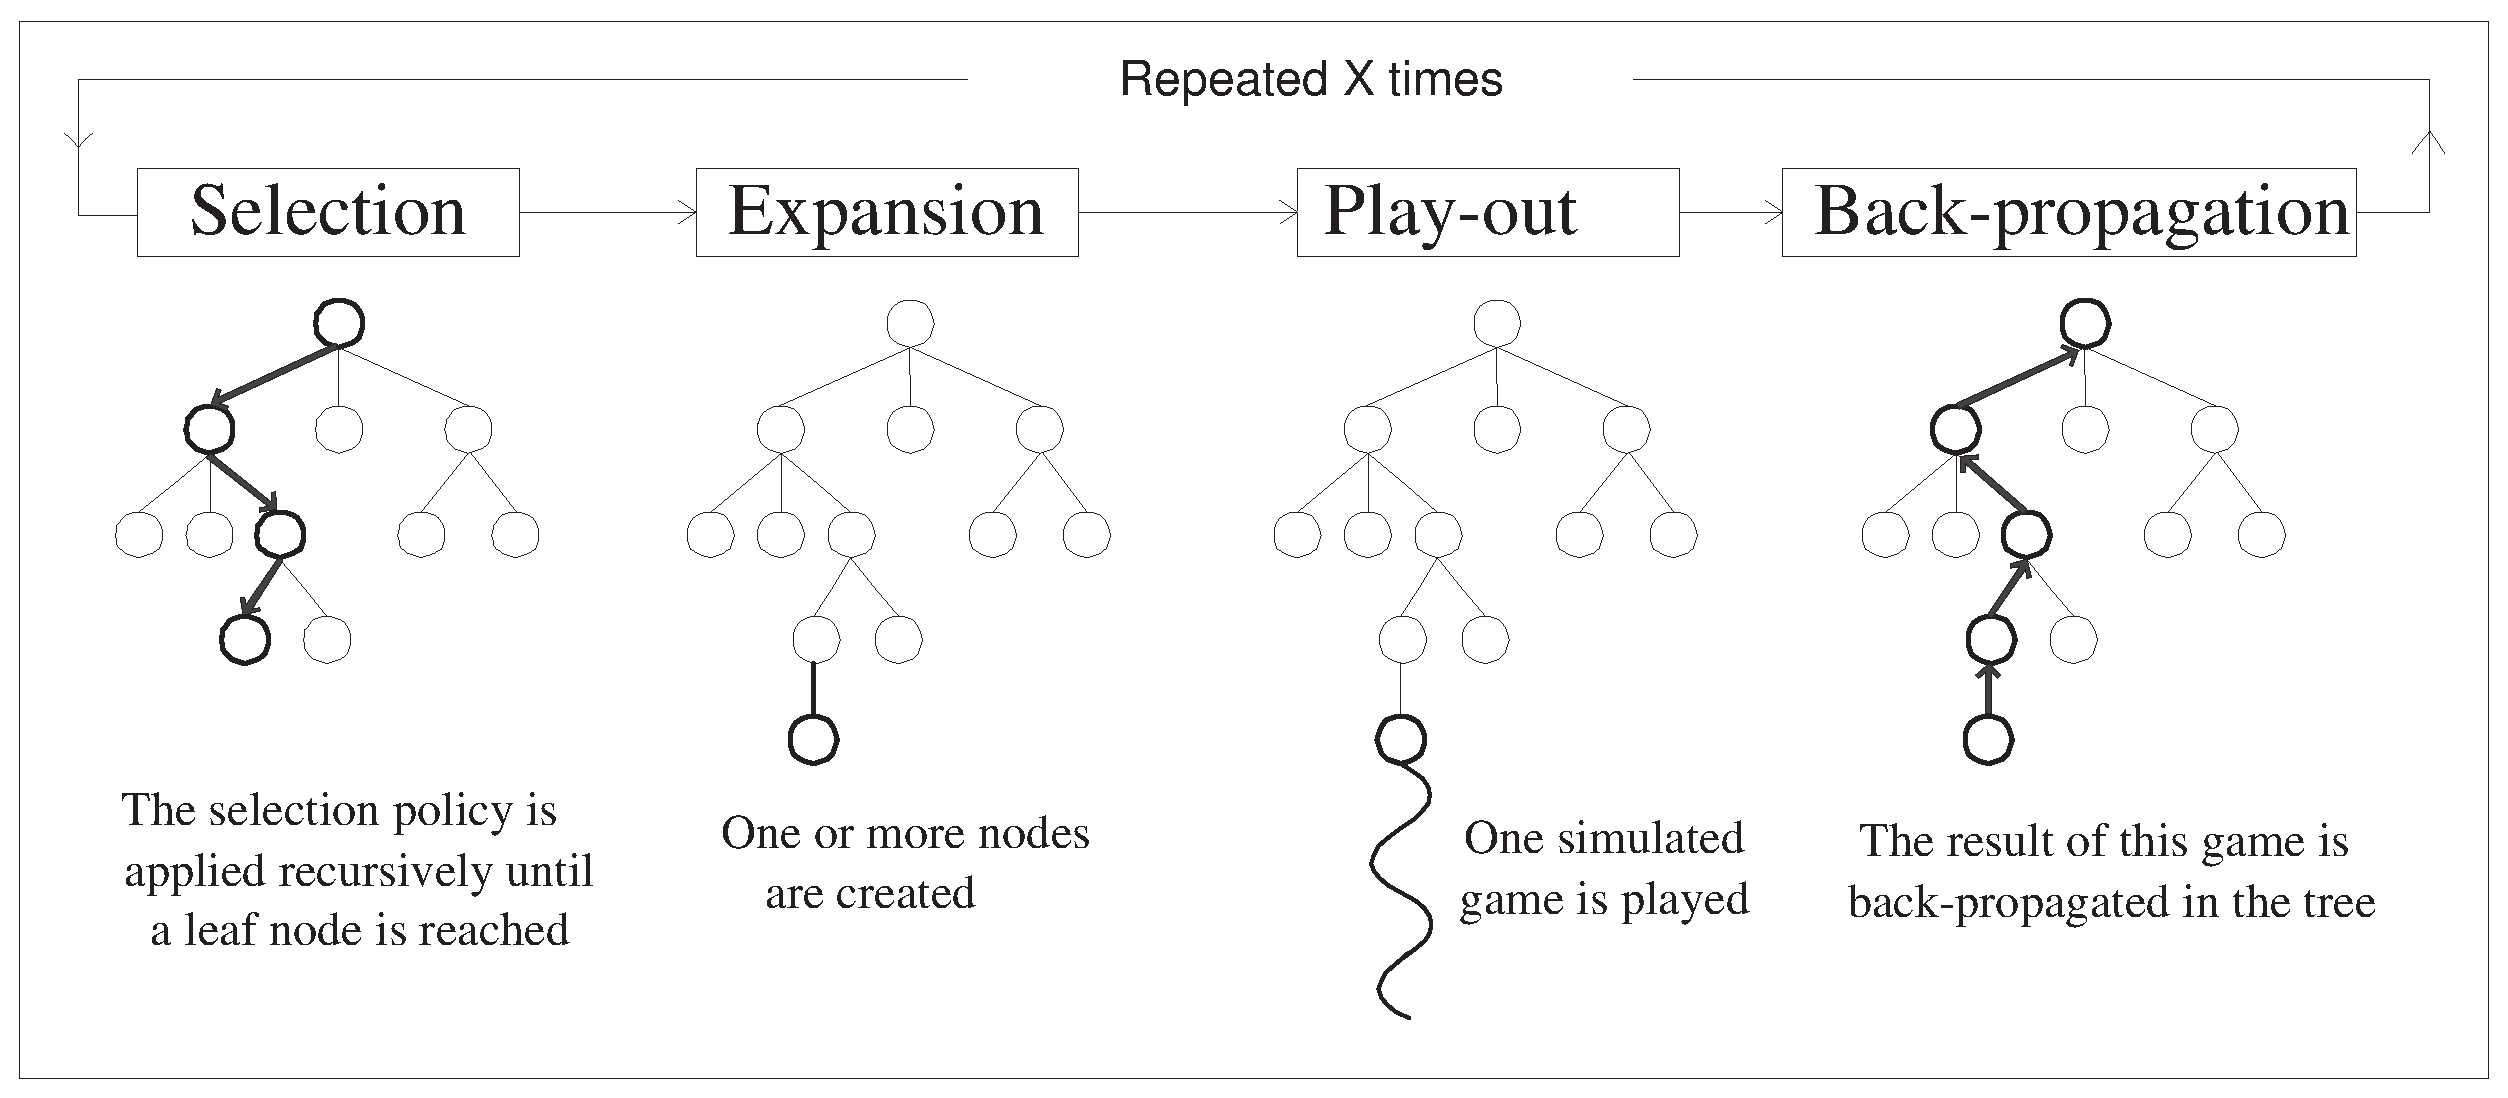
\includegraphics[width=.45\textwidth]{img/figure1.eps}
	\caption{Strategic steps of Monte-Carlo Tree Search \cite{chaslot2008progressive}.}
	\label{fig:mcts-algorithm}
\end{figure}

\section{Assessing play-out quality}
\label{sec:poqual}

\begin{figure}[ht]
	\centering
	\includegraphics[width=.3\textwidth]{img/figure2.png}
	\caption{A single MCTS simulation \cite{finnsson2010learning}.}
	\label{fig:mcts-simulation}
\end{figure}

The first, straightforward assessment of a play-out's quality is the length of the game played. Consider a single MCTS simulation as depicted in Figure \ref{fig:mcts-simulation}, here we can define two seperate distances: 
\begin{enumerate}
\item The number of moves from the root $S$ to the expanded leaf $N$, $d_{SN}$,
\item The number of moves required to reach $T$, the terminal state, from $N$ during play-out $p_{NT}$.
\end{enumerate}
The length of the simulation is defined as the sum of these distances $m_{ST} = d_{SN} + p_{NT}$, i.e. the total number of moves made by both players to reach the terminal state of the game from the current gamestate.

Considering that, in Monte-Carlo methods a random element is present in simulations, each move played increases the uncertainty of the final result. The most important benefit of using this information is that it can be obtained independent of the domain. Unless the game has a fixed-length, the variance of the length of a play-out can be informative in determining its quality.

%-------------------------------------------------------------------
\section{Quality-based play-out rewards}
Alter rewards, centered around $r_t$ using sigmoid. Sigmoids are great, i love them, here's why!
\begin{figure}[ht]
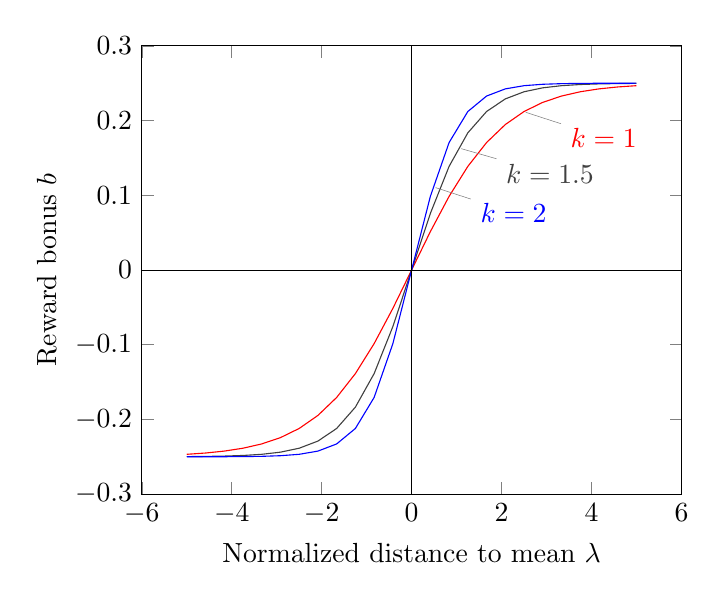
\begin{tikzpicture}
\pgfplotsset{compat=1.9}
  \begin{axis}[
	ylabel = Reward bonus $b$,
    xlabel = Normalized distance to mean $\lambda$,
  	axis equal image=false 
  	]
    \addplot[red, mark=none] {.5/(1+e^(-x)) - .25} node [pos=0.75,pin={-10:$k=1$},inner sep=0pt]{};
    \addplot[darkgray, mark=none] {.5/(1+e^(-1.5*x)) - .25} node [pos=0.607,pin={-10:$k=1.5$},inner sep=0pt]{};
    \addplot[blue, mark=none] {.5/(1+e^(-2*x)) - .25} node [pos=0.55,pin={-10:$k=2$},inner sep=0pt]{};
    \draw[ultra thin] (axis cs:\pgfkeysvalueof{/pgfplots/xmin},0) -- (axis cs:\pgfkeysvalueof{/pgfplots/xmax},0);
	\draw[ultra thin] (axis cs:0,\pgfkeysvalueof{/pgfplots/ymin}) -- (axis cs:0,\pgfkeysvalueof{/pgfplots/ymax}); 
  \end{axis}
\end{tikzpicture}
    \caption{Rewards resulting from sigmoid functions centered around 0.}
	\label{fig:sigmoids}
\end{figure}
\subsection{Relative Bonus}
Alter the rewards based on $m_{ST}$
\subsection{Qualitative Bonus}
Alter the reward based on the quality of the terminal state. Different heuristics per game.

%-------------------------------------------------------------------
\section{Algorithm}
Explain all the alterations to standard MCTS
\begin{algorithm2e}[ht]
\setstretch{1.15}
  {\bf MCTS}(node $n_p$, cumulative node depth $d_{S, n_p}$):\;
  \pushline
    \If{isLeaf($n_p$)}{Expand($n_p$)}
    Select a child $n_i$ that maximizes $X_i$ from Eq.~\ref{eq:uct} 	\;
    $d_{S, n_i} \gets d_{S, n_p} + 1$								\;
    \eIf{$visits(n_i) = 0$}{
    	$\{q_t, p_{n_it}, r_t\} \gets$ Playout$(n_i)$ 					\;			\label{alg:results}
    	$m_{St} \gets d_{S, n_i} + p_{n_it}$									\;
    	\If{enabled$(rb)$}{
    		$\tilde{r_t} \gets r_t + \sgn(r_t) \times$ BONUS$(\bar{M} - m_{St}, s_m)$ 		\;
    		Update $\bar{M}$ and $s_m$ with $m_{St}$						\;
		}
		\If{enabled$(qb)$} {
    		$\tilde{r_t} \gets r_t + \sgn(r_t) \times$ BONUS$(q_t -\bar{Q}, s_q)$ 		\;
    		Update $\bar{Q}$ and $s_q$ with $q_t$ 						\;
    	}
    	Update $n_i$ with $\tilde{r_t}$
    }{
    	$\tilde{r_t}$ = -MCTS($c_i$, $d_{S, n_i})$)								\; 
    }
    Update $n_p$ with $\tilde{r_t}$													\;
   \popline
    {\bf return} $\tilde{r_t}$													\;
  	\;
    {\bf BONUS}(distance to mean $\delta$, std. dev. $s$):			\;
    \pushline
    	$\lambda \gets \frac{\delta}{s}$								\;
    	$b \gets \frac{0.5}{1+\exp(-K\lambda)} - 0.25$					\;
    \popline
    \bf{return} $b$														\;
  \vspace{0.3cm}
  \caption{Pseudo-code of the MCTS and BONUS functions \label{alg}}
\end{algorithm2e}

%-------------------------------------------------------------------
\section{Experiments}
Experiments run on 5 different two player boardgames.
\subsection{Experimental setup}
Describe setup of experiments, k's used, c's used.

\subsection{Results}
- Results UCT vs RB
- Results UCT vs QB
- Results UCT vs RB + RB
- Results RB vs QB
- Graph of K's / UCT C's

%-------------------------------------------------------------------
\section{Conclusion}
Relative bonus - interesting because requires no domain knowledge, works best in games with long play-outs.
QB works in all domains, but requires domain knowledge, nonetheless, even using simple evaluation of the terminal state improved results considerably.

RB especially interesting for General Game Playing (GGP), where knowledge of games is sparse. RB improves results without domain-dependent knowledge.

Would be interesting to determine if RB/QB could improve results in non-game domains.

%-------------------------------------------------------------------
\bibliography{references}
\end{document}